\documentclass[11pt,a4paper]{report}%especifica o tipo de documento que tenciona escrever: carta, artigo, relatório... neste caso é um relatório
% [11pt,a4paper] Define o tamanho principal das letras do documento. caso não especifique uma delas, é assumido 10pt
% a4paper -- Define o tamanho do papel.
\usepackage{float}
\usepackage[portuges]{babel}%Babel -- irá activar automaticamente as regras apropriadas de hifenização para a língua todo o
                                   %-- o texto gerado é automaticamente traduzido para Português.
                                   %  Por exemplo, “chapter” irá passar a “capítulo”, “table of contents” a “conteúdo”.
                                   % portuges -- específica para o Português.
\usepackage[utf8]{inputenc} % define o encoding usado texto fonte (input)--usual "utf8" ou "latin1

\usepackage{graphicx} %permite incluir graficos, tabelas, figuras
\usepackage{url} % para utilizar o comando \url{}
\usepackage{enumerate} %permite escolher, nas listas enumeradas, se os iems sao marcados com letras ou numeros-romanos em vez de numeracao normal

%\usepackage{apalike} % gerar biliografia no estilo 'named' (apalike)

\usepackage{color} % Para escrever em cores

\usepackage{multirow} %tabelas com multilinhas
\usepackage{array} %formatação especial de tabelas em array

\usepackage[pdftex]{hyperref} % transformar as referências internas do seu documento em hiper-ligações.

%Exemplos de fontes -- nao e vulgar mudar o tipo de fonte
%\usepackage{tgbonum} % Fonte de letra: TEX Gyre Bonum
%\usepackage{lmodern} % Fonte de letra: Latin Modern Sans Serif
%\usepackage{helvet}  % Fonte de letra: Helvetica
%\usepackage{charter} % Fonte de letra:Charter

\definecolor{saddlebrown}{rgb}{0.55, 0.27, 0.07} % para definir uma nova cor, neste caso 'saddlebrown'

\usepackage{listings}  % para utilizar blocos de texto verbatim no estilo 'listings'
%paramerização mais vulgar dos blocos LISTING - GENERAL
\lstset{
	basicstyle=\small, %o tamanho das fontes que são usadas para o código
	numbers=left, % onde colocar a numeração da linha
	numberstyle=\tiny, %o tamanho das fontes que são usadas para a numeração da linha
	numbersep=5pt, %distancia entre a numeração da linha e o codigo
	breaklines=true, %define quebra automática de linha
    frame=tB,  % caixa a volta do codigo
	mathescape=true, %habilita o modo matemático
	escapeinside={(*@}{@*)} % se escrever isto  aceita tudo o que esta dentro das marcas e nao altera
}
%
%\lstset{ %
%	language=Java,							% choose the language of the code
%	basicstyle=\ttfamily\footnotesize,		% the size of the fonts that are used for the code
%	keywordstyle=\bfseries,					% set the keyword style
%	%numbers=left,							% where to put the line-numbers
%	numberstyle=\scriptsize,				% the size of the fonts that are used for the line-numbers
%	stepnumber=2,							% the step between two line-numbers. If it's 1 each line
%											% will be numbered
%	numbersep=5pt,							% how far the line-numbers are from the code
%	backgroundcolor=\color{white},			% choose the background color. You must add \usepackage{color}
%	showspaces=false,						% show spaces adding particular underscores
%	showstringspaces=false,					% underline spaces within strings
%	showtabs=false,							% show tabs within strings adding particular underscores
%	frame=none,								% adds a frame around the code
%	%abovecaptionskip=-.8em,
%	%belowcaptionskip=.7em,
%	tabsize=2,								% sets default tabsize to 2 spaces
%	captionpos=b,							% sets the caption-position to bottom
%	breaklines=true,						% sets automatic line breaking
%	breakatwhitespace=false,				% sets if automatic breaks should only happen at whitespace
%	title=\lstname,							% show the filename of files included with \lstinputlisting;
%											% also try caption instead of title
%	escapeinside={\%*}{*)},					% if you want to add a comment within your code
%	morekeywords={*,...}					% if you want to add more keywords to the set
%}

\usepackage{xspace} % deteta se a seguir a palavra tem uma palavra ou um sinal de pontuaçao se tiver uma palavra da espaço, se for um sinal de pontuaçao nao da espaço

\parindent=0pt %espaço a deixar para fazer a  indentação da primeira linha após um parágrafo
\parskip=2pt % espaço entre o parágrafo e o texto anterior

\setlength{\oddsidemargin}{-1cm} %espaço entre o texto e a margem
\setlength{\textwidth}{18cm} %Comprimento do texto na pagina
\setlength{\headsep}{-1cm} %espaço entre o texto e o cabeçalho
\setlength{\textheight}{23cm} %altura do texto na pagina

% comando '\def' usado para definir abreviatura (macros)
% o primeiro argumento é o nome do novo comando e o segundo entre chavetas é o texto original, ou sequência de controle, para que expande
\def\darius{\textsf{Darius}\xspace}
\def\antlr{\texttt{AnTLR}\xspace}
\def\pe{\emph{Publicação Eletrónica}\xspace}
\def\titulo#1{\section{#1}}    %no corpo do documento usa-se na forma '\titulo{MEU TITULO}'
\def\super#1{{\em Supervisor: #1}\\ }
\def\area#1{{\em \'{A}rea: #1}\\[0.2cm]}
\def\resumo{\underline{Resumo}:\\ }

%\input{LPgeneralDefintions} %permite ler de um ficheiro de texto externo mais definições

\title{Projeto de Infraestruturas de Centro de Dados\\
        1º/4º ano MEI/MIEI\\
       \textbf{Escalabilidade de Infraestruturas Telemetria de Infraestruturas}\\ Relatório de Desenvolvimento
       } %Titulo do documento
%\title{Um Exemplo de Artigo em \LaTeX}
\author{Isaac Paulo Betuel Mabiala\\ (pg41074@alunos.uminho.pt) \and João Paulo Oliveira de Andrade Marques \\ (a81826@alunos.uminho.pt) \and José André Martins Pereira\\ (a82880@alunos.uminho.pt) \and Ricardo André Gomes Petronilho\\ (a81744@alunos.uminho.pt)
       } %autores do documento
\date{\today} %data

\begin{document} % corpo do documento

\begin{figure}
    \centering
    
\includegraphics{imagens/uminho.png}
\end{figure}

\maketitle % apresentar titulo, autor e data

\tableofcontents % Insere a tabela de indice
%\listoffigures % Insere a tabela de indice figuras
%\listoftables % Insere a tabela de indice tabelas

\chapter{Introdução} \label{chap:intro} %referência cruzada

\hspace{5mm} No âmbito da Unidade Curricular de Infraestruturas de Centro de Dados, foi-nos proposto o desenvolvimento de uma arquitetura para um sistema da aplicação \textbf{Tucano}. 

\hspace{5mm} Ao longo deste relatório abordam-se as fases de desenho e desenvolvimento da arquitetura, explicação e disponibilidade da mesma, quais os possíveis pontos de falha e testes de carga realizados sobre a mesma, bem como análise dos resultados obtidos em cada fase.


\hspace{5mm} Inicialmente, faz-se uma contextualização do problema, bem como uma análise da aplicação \textbf{Tucano}, para se entender a arquitetura da aplicação, bem como as suas dependências. 
 
 
\hspace{5mm} De seguida, descreve-se a arquitetura implementada, decisões realizadas para se atigirem os objetivos referidos acima. 


\hspace{5mm} A identificação de \textbf{SPOFS}, ou seja, pontos críticos da arquitetura implementada, e as soluções encontradas, para reduzir o impacto dos mesmos.


\hspace{5mm} Por fim, e não menos importante, apresenta-se uma avaliação do desempenho dos sitema, para uma melhor definição da arquitetura, a nível da disponibilidade dos diferentes componentes, bem como testes de carga. 
\chapter{Descrição/perceção do Problema}

\hspace{5mm} Neste capítulo faz-se uma descrição/contextualização do problema em análise, abordando-se os objetivos pretendidos.

\section{Objetivos}
\hspace{5mm} Os principais objetivos deste projeto concentram-se no desenvolvimento de uma arquitetura, com infraestruturas que promovam alta disponibilidade e desempenho, sendo necessário planeamento e deployment para a concretização do mesmo. Após a construção desta arquitetura, tem-se que perceber, os pontos críticos da mesma, e soluções para reduzir o impacto desses mesmos pontos.

\section{Análise da aplicação}

\hspace{5mm} A análise da arquitetura da aplicação torna-se importante para melhor perceção da divisão dos diferentes componentes. Deste modo, com uma análise do relatório elaborado pelos criadores da aplicação, conseguiu-se perceber que a aplicação está divida em dois subsistemas, \textbf{frontend} e \textbf{backend}.

\hspace{5mm} O frontend, utiliza uma biblioteca base do ReactJS em conjunto com componentes na sua maioria do Semantic UI, tendo um servidor em constante execução.

\hspace{5mm} O backend, é composto por uma API utilizando a framework Phoenix escrita em Elixir que por sua vez compila para a BEAM (Erlang virtual machine) garantindo assim de forma fácil a escalabilidade da plataforma. Do mesmo modo, que o frontend, o backend consiste num servidor aplicacional, que interage com o servidor de base de dados de PostgreSQL.

\section{Instalação e Configuração}
\hspace{5mm} Com a finalidade de complementar a análise feita anteriormente, e utilizando a documentação disponibilizada pela equipa que desenvolveu o \textbf{Tucano}, procedeu-se à instalação da mesma, seguindo o guião de instalação.

\hspace{5mm} Deste modo, o grupo decidu instalar inicialmente todos os componentes na máquina \emph{localhost}, para entender as dependências, e configurações necessárias para o bom funcionamento da aplicação. Os processos seguidos nesta instalação, serão realizados novamente, no deployment do \textbf{Tucano}, para a arquitetura apresentada no decorrer do relatório. 

Assim, conclui-se que o projeto foi importante para uma melhor perceção e aprofundamento dos conhecimentos obtidos nas aulas teóricas, bem como entender como as aplicações de hoje em dia estão preparadas para falhas que acontecem diariamente.
\chapter{Desenvolvimento} \label{chap:desen}

\hspace{5mm} Nesta secção serão abordadas as fases de implementação da arquitetura desenvolvida, problemas e respetivas soluções para a implementação, alguns dos pontos críticos que foram encontrados e possíveis soluções, e ainda os resultados obtidos através de testes de carga.

\section{Arquitetura implementada} \label{sec:arqimp}

\hspace{5mm} A arquitetura implementada divide-se em 3 partes: os
LVS, o Cluster e o DRBD.

\subsection{LVS} \label{subsec:lvs}

\hspace{5mm} Inicialmente começou-se por configurar duas máquinas LVSs - \textbf{Linux Virtual Server} - juntamente com três máquinas WS - Web Server.

\hspace{5mm} Os pedidos dos clientes são recebidos por um dos LVS na placa \textbf{NAT} com o endereço IP \textbf{192.168.64.168}, sendo de seguida reencaminhados para um dos WS existindo assim \textbf{balanceamento e caso um dos WS não esteja funcional o pedido é servido por outro WS}. No caso dos LVSs estão todos ligados mas \textbf{apenas um se encontra ativo em cada momento}, ou seja, os pedidos são sempre redirecionados para um LVS e caso esse falhe um dos outros é ativo para continuar a responder aos pedidos que chegam.

\begin{figure}[H]
	\centering
	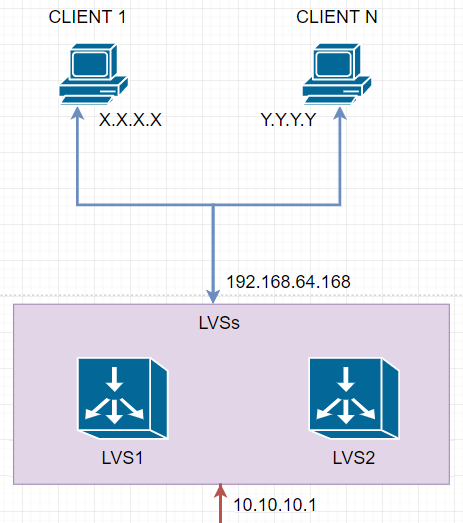
\includegraphics[scale=0.45]{imagens/client-lvs.PNG}
	\caption{Conexões dos Clientes aos LVs.}
	\label{img:pag}
\end{figure}

\hspace{5mm} Desta forma o serviço de FrontEnd é hóspedado pelos respetivos WSs.

\hspace{5mm} A conectividade entre os LVSs e os WSs é efetuado através de uma rede \textbf{isolada} na gama de endereços IP \textbf{10.10.10.0/24}. Os LVSs são identificados pelo endereço \textbf{10.10.10.1} uma vez que é o \textbf{gateway} desta rede, isto é, as conexões que todas as máquinas nesta rede efetuarem são mapeadas pelo LVS, isto apenas é possível porque \textbf{em cada momento só um dos LVS é que se encontra ativo}.

\hspace{5mm} Assim foi definido no ficheiro \textbf{
/etc/keepalived/keepalived.conf} do LVS o mapeamento das conexões. No caso da nossa arquitetura foram definidas rotas para a porta \textbf{80} (FrontEnd) e para a \textbf{4000} (BackEnd).

\hspace{5mm} A necessidade de ter definido a porta 4000 para acesso ao BackEnd deve-se ao facto de alguns pedidos internos do FrontEnd necessitarem de acesso ao BackEnd. 

\hspace{5mm} Idealmente os nodos do cluster (\ref{subsec:cluster}) deveriam estar numa rede \textbf{diferente} da rede isolada criada para a comunicação entre os LVSs e os WSs, mas devido a dificuldades de implementação estes encontram-se na mesma rede, existindo assim conetividade. Note-se que os WSs \textbf{não acedem diretamente aos nodos do cluster}, apenas comunicam com os LVSs, e os mesmos redirecionam os pacotes para os respetivos nodos.

\begin{figure}[H]
	\centering
	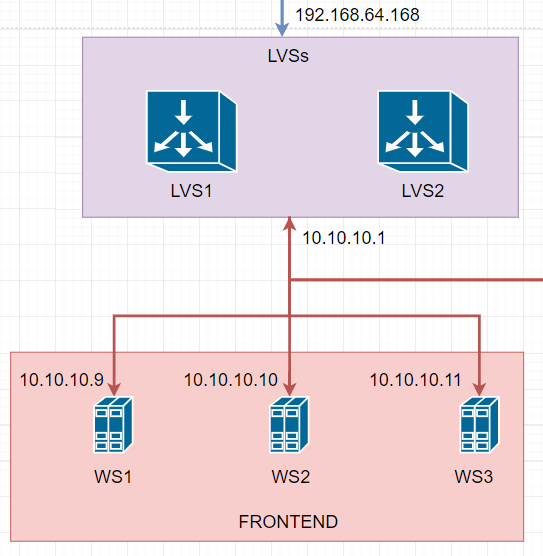
\includegraphics[scale=0.5]{imagens/lvs-ws.PNG}
	\caption{Ligações entre os LVSs e os WSs.}
	\label{img:pag}
\end{figure}


\subsection{Cluster} \label{subsec:cluster}

\hspace{5mm} O cluster permite que os serviços expostos pelo mesmo tenham \textbf{alta disponibilidade}. No âmbito da nossa arquitetura o cluster é constítuido por dois nodos: \textbf{cl1} e \textbf{cl2}; com os respetivos endereços IP: \textbf{10.10.10.8} e \textbf{10.10.10.9}; estando conectados à rede isolada \textbf{10.10.10.0/24} para que os LVSs tenham conectividade ao cluster tal como referido na secção anterior.

\hspace{5mm} Com a ajuda das ferramentas: \textbf{pcs}, \textbf{pacemaker} e \textbf{fence-agents-all}; fornecidas pela equipa \href{https://www.redhat.com/}{Red Hat} foi configurado o cluster sendo definidos dois serviços: o serviço \textbf{tupi} (backend) e o serviço \textbf{postgresql} (base de dados). Para cada um dos serviços foram criados três \textbf{recursos}: \textbf{endereço de IP virtual}, \textbf{filesystem} e o \textbf{serviço efetivamente a hospedar}. O endereço de IP virtual é utilizado para que as máquinas LVSs externas ao cluster consigam conectar-se ao respetivo serviço. O endereço é virtual uma vez que quando é efetuado um pedido a um serviço, o software do cluster faz o encaminhamento do pedido para o nodo em que se encontra disponível, desta forma \textbf{não existe uma conexão direta a um nodo do cluster}.

\hspace{5mm} O serviço postgresql foi construído com três recursos, já referidos acima, sendo que o endereço de IP virtual é o \textbf{10.10.10.21}. O filesystem monta a partição \textbf{/dev/mapper/mpatha2} (partição 2 do DRBD) na pasta \textbf{/mnt/db}. Por fim para a configuração do servidor foi necessário alterar a pasta onde o serviço postgresql inicia a base dados por padrão, para isso, alteramos a variável \textbf{PGDATA} no ficheiro \textbf{/var/lib/pgsql/data/postgres.conf} para a pasta onde foi montado o filesystem da base de dados - \textbf{/mnt/db}. Desta forma quando o serviço postgresql é inicializado, \textbf{automaticamente inicia o servidor com os ficheiros corretos}. Note-se que o software do cluster escolhe automaticamente qual o nodo a hospedar um determinado serviço, desta forma, os serviços tupi (backend) e postgresql \textbf{podem estar em nodos diferentes}, por exemplo, o nodo cl1 pode hospedar o serviço tupi e o nodo cl2 o serviço postgresql, desta forma para que o serviço tupi consiga aceder ao postgresql, o mesmo tem de \textbf{permitir conexões externas}. Assim alteramos a variável \textbf{listen\_addresses} no ficheiro \textbf{/mnt/db/postgresql.conf} para - \textbf{*} - e no ficheiro \textbf{/mnt/db/pg\_hba.conf} introduzimos a linha - \textbf{host all all 10.10.10.1/24 md5} - desta forma permite-se conexões ao servidor da base de dados provenientes da rede isolada.

\hspace{5mm} O serviço tupi (backend) foi construído do mesmo modo que o serviço do postgresql, sendo que o endereço de IP virtual é o \textbf{10.10.10.20}. O filesystem monta a partição \textbf{/dev/mapper/mpatha1} (partição 1 do DRBD) na pasta \textbf{/mnt/backend}. Por fim para a configuração do servidor foi necessário criar o ficheiro \textbf{/etc/systemd/system/tupi.service} que especifica na variável \textbf{ExecStart} o script a correr quando é inicializado o serviço tupi com o programa \textbf{systemd}. Neste caso o script que é corrido é o ficheiro \textbf{/mnt/backend/tupi/tupi.sh}.

\begin{figure}[H]
	\centering
	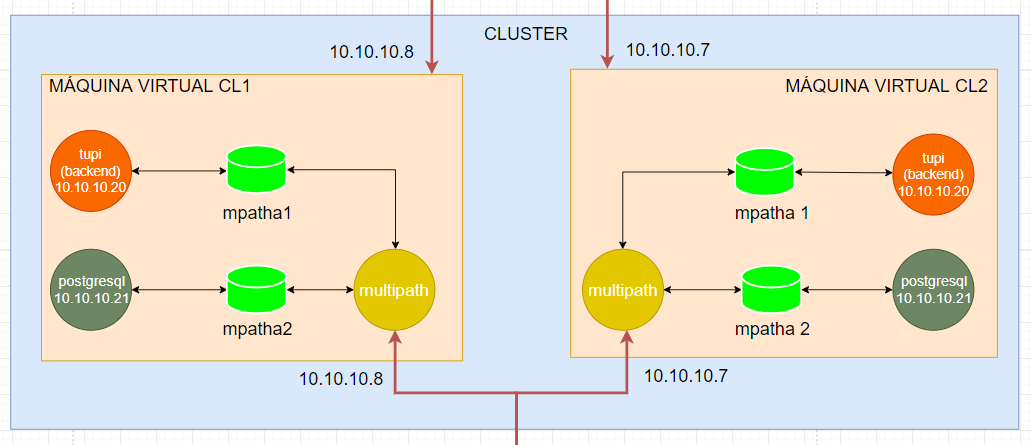
\includegraphics[scale=0.6]{imagens/cluster.PNG}
	\caption{Cluster com os respetivos nodos e serviços.}
\end{figure}



\subsection{DRBD} \label{subsec:drbd}

\hspace{5mm} Na arquitetura desenvolvida neste projeto foi implementado um \textbf{DRDB} - Distributed Replicated Block Device.

\hspace{5mm} No processo de configuração do DRBD foi utilizado o protocolo \textbf{iSCSI} que é um protocolo IP para conectar entre si instalações de armazenamento de dados. Permite o controlo de dispositivos de armazenamento através de comandos \textbf{SCSI} - Small Computer Systems Interface – pela camada TCP/IP (pela rede). Desta forma quem utilizar o protocolo iSCSI conecta-se a um dispositivo remoto (na rede) da mesma maneira que a um dispositivo periférico local (ex: pen usb) tendo total \textbf{abstração da conexão remota}. A arquitetura deste protocolo consiste em iSCSI clients (nodos do cluster) e iSCSI targets (máquinas drbd1 e drbd2).

\hspace{5mm} Foi também utilizado o programa \textbf{multipath} que configura múltiplas rotas entre um servidor e seus dispositivos de armazenamento remotos de forma a \textbf{agregar todas as rotas num único caminho} para o dispositivo.

\hspace{5mm} Para existir comunicação entre as máquinas DRBDs e dos nodos do cluster foi utilizada a rede isolada 10.10.10.0/24, sendo que a máquina drbd1 está a usar o endereço IP 10.10.10.41 e a drbd2 utiliza o endereço IP 10.10.10.40.

\hspace{5mm} No caso de \textbf{failover} de um dos DRBDs o sistema \textbf{continua a funcionar pois ambas as máquinas DRBD são DRBD primários}. Quando a máquina DRBD que falhou voltar ao ativo novamente faz sincronização de dados com a DRBD que continuou a sua execução enquanto esta falhou.

\begin{figure}[H]
	\centering
	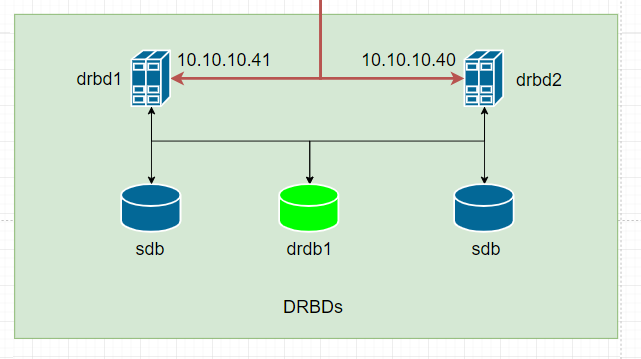
\includegraphics[scale=0.7]{imagens/drbd.PNG}
	\caption{Arquitetura do DRBD.}
	\label{img:pag}
\end{figure}

\begin{figure}[H]
	\centering
	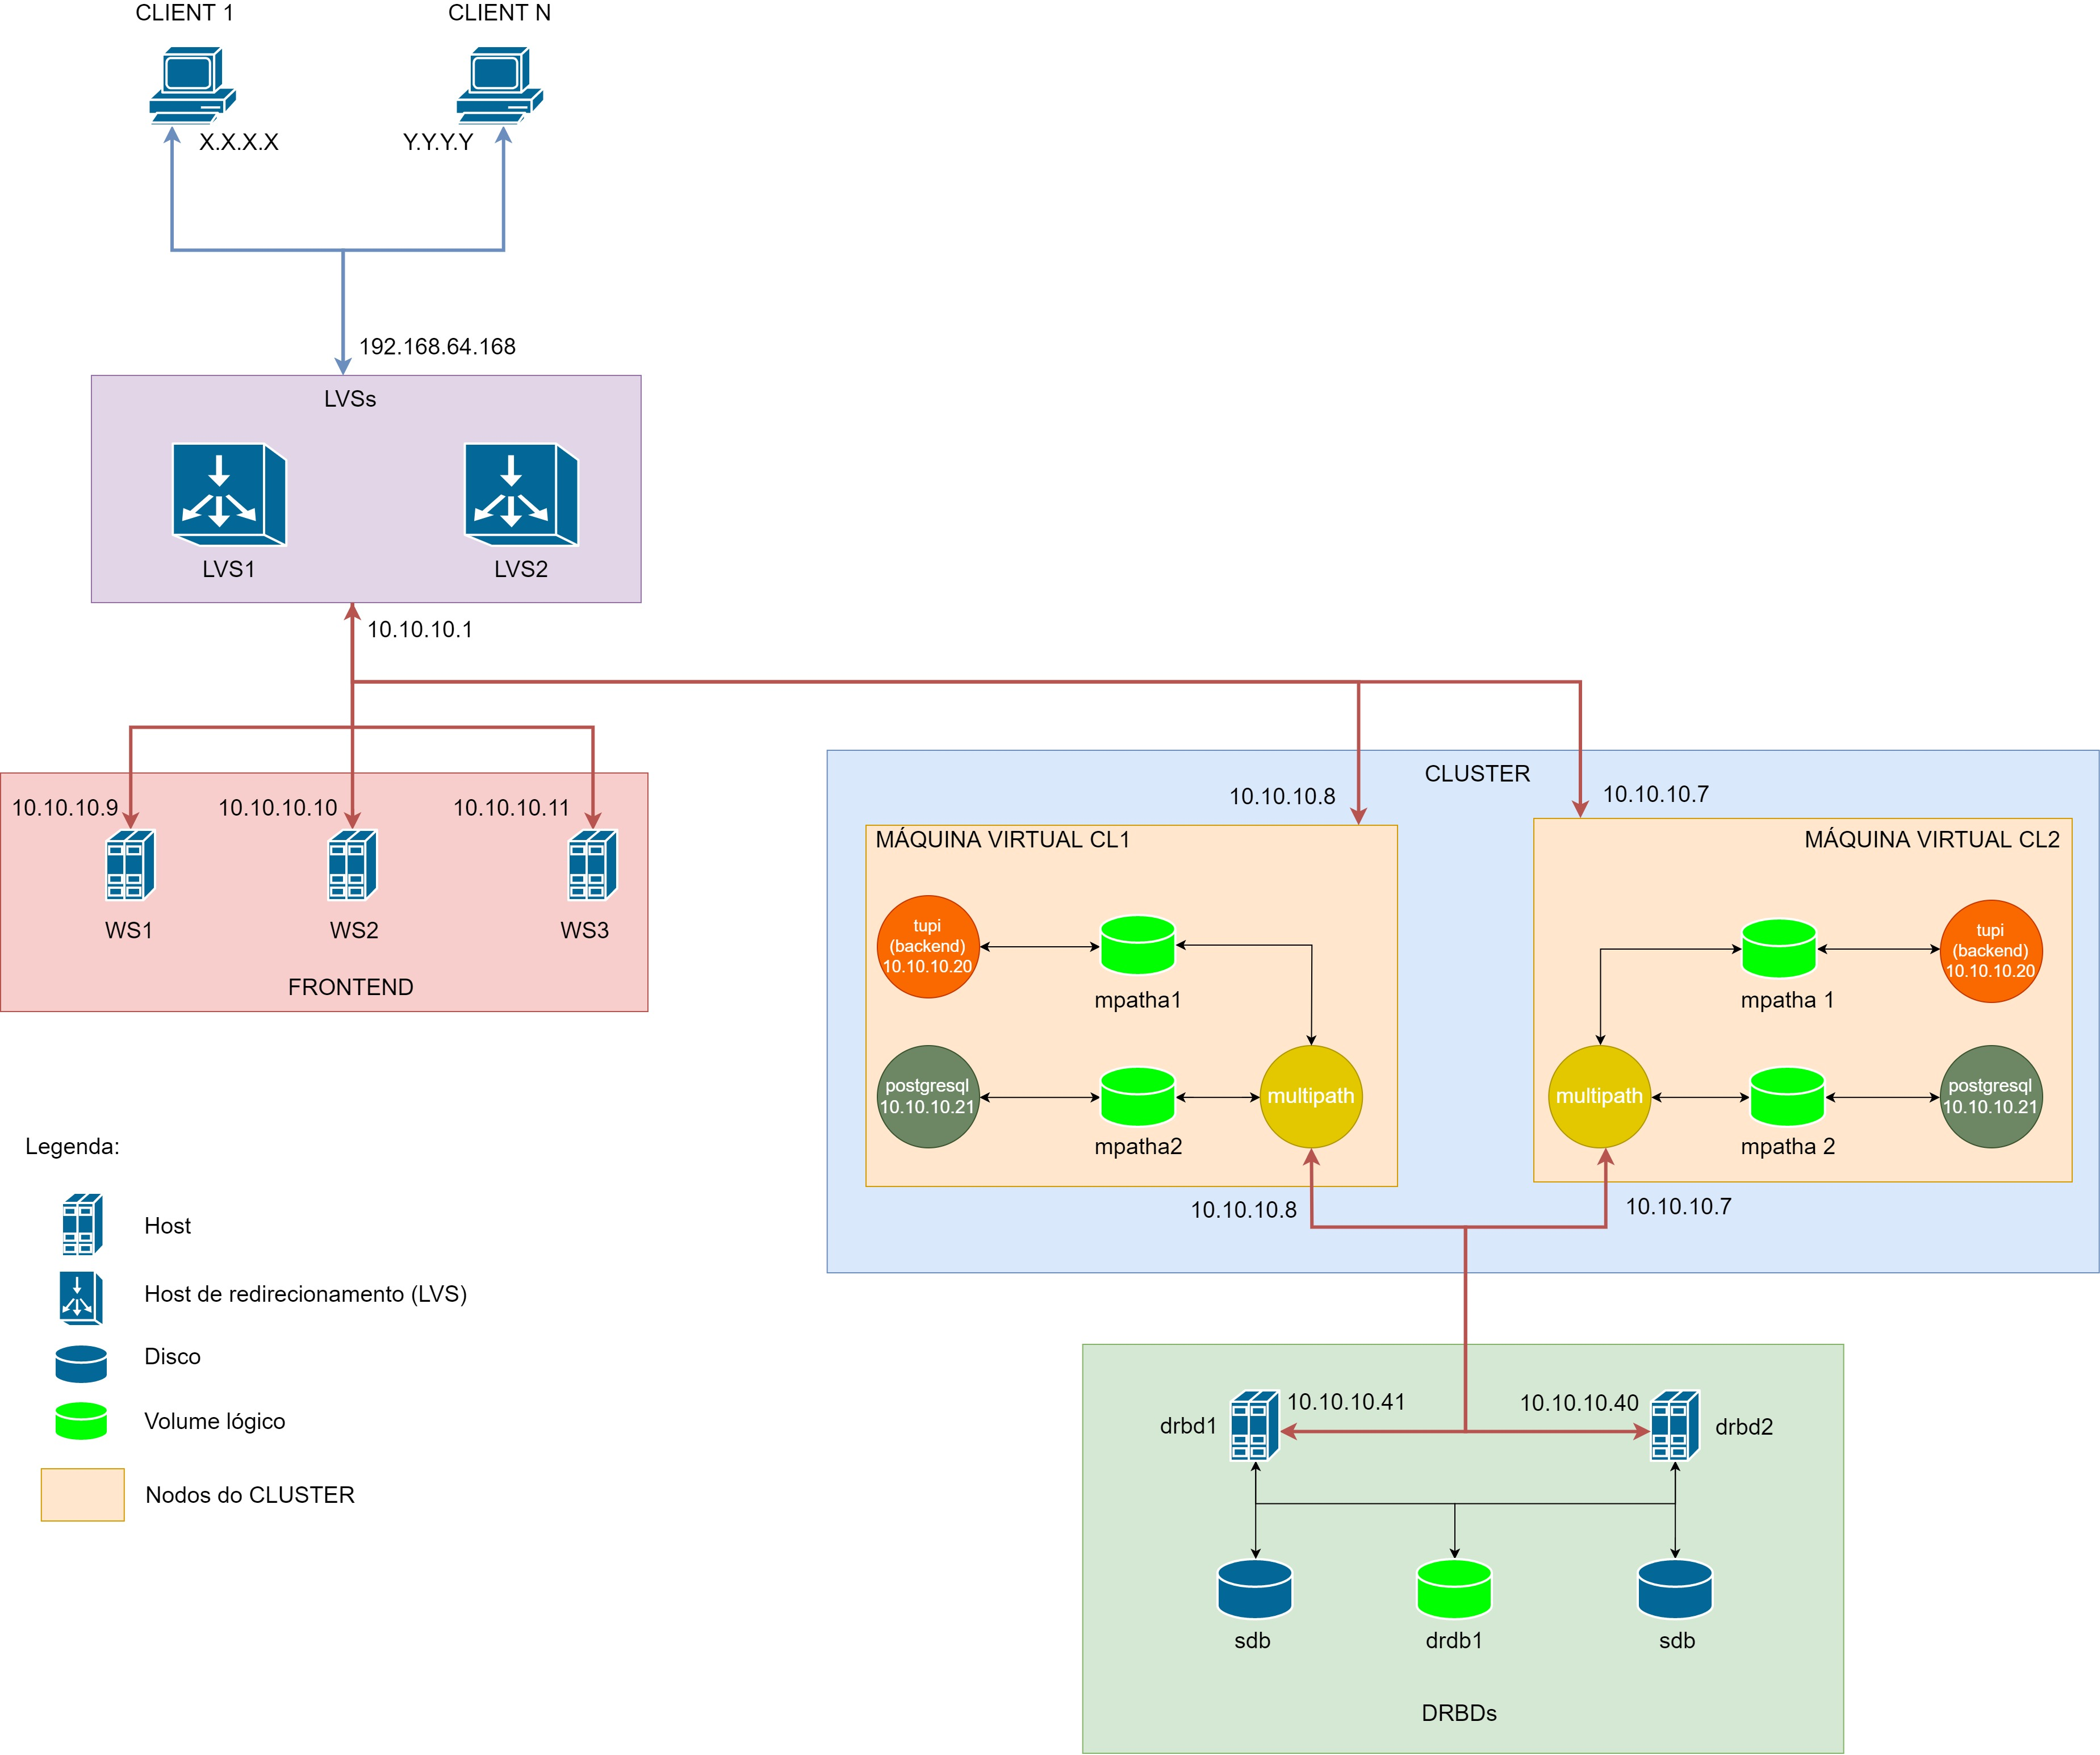
\includegraphics[scale=0.14]{imagens/arquitetura.jpg}
	\caption{Arquitetura da infraestrutura.}
	\label{img:pag}
\end{figure}

\section{Identificação de SPOFs} \label{sec:idenSPOF}

\hspace{5mm} Os possíveis pontos de rutura da arquitetura são: \textbf{LVS}, \emph{web services} , \textbf{DRBD} e \textbf{Cluster}. Importante referir, que existirão sempre estes pontos de rutura, pois não se consegue evitar a 100\%, visto que os recursos não são ilimitados, mas sim reduzir a probabilidade das ruturas acontecerem. O \textbf{LVS} pode provocar a quebra do sistema, pois consiste no ponto de entrada no mesmo. Deste modo, a sua falta, torna todo o sistema inutilizável. Como solução para este ponto crítico, a equipa decidiu, como já referido anteriormente, ter uma segunda máquina \textbf{LVS}, pronta para entrar em funcionamento em caso de falha.

\hspace{5mm} Do mesmo modo, os \emph{web services}, máquinas com o servidor frontend, são um ponto de rutura, pois com apenas um servidor, em caso da sua falha, o sistema fica inutilizável, pois necessita-se da interface gráfica para utilização da aplicação. Assim, o grupo decidiu colocar três máquinas com os \emph{web services}, ou seja, podem falhar até duas máquinas, e o sistema mantém-se em funcionamento. Com a adição destas três máquinas, também garante-se a distribuição da carga, reduzindo assim, a possibilidade de falha das mesmas.

\hspace{5mm} Em relação ao cluster, este também se torna um ponto crítico, pois agrega os serviços de backend, e base de dados, cruciais ao funcionamento do sistema. Deste modo, com a finalidade de garantir a disponibilidade destes mesmos serviços, decidiu-se conter dois nodos no cluster, tal como já foi referido, sendo que, os serviços em caso de falha de um servidor, automaticamente, se ativam em outro nodo do mesmo, logo, consegue-se ter até a um máximo de uma falha no cluster, e continuar-se em funcionamento. O ideal seria adicionar mais nodos ao cluster, para reduzir a probabilidade de rutura, no entanto, face aos recursos, apenas foi possível colocar dois nodos.

\hspace{5mm} Por fim, e não menos importante, têm-se o ponto de rutura do \textbf{DRBD}, responsável pelos dados dos serviços do \textbf{Cluster}, logo percebe-se a importância e os problemas, que a falha do mesmo, causa em todo o sistema. Assim, a própria arquitetura do \textbf{DRBD} está preparada para falhas, garantindo-se que na falta de uma das máquinas do mesmo, os dados dos serviços estão salvaguardados e mantidos em funcionamento.

\section{Avaliação do desempenho do sistema} \label{sec:avaldesemp}

\hspace{5mm} Para a avaliação de desempenho do sistema foram realizados vários testes para garantir a alta disponibilidade e fiabilidade do mesmo. Para tal foram realizados testes de carga ao FrontEnd e ao BackEnd, foram ainda realizados testes ao nível de disponibilidade do sistema, caso de failover do LVS ou dos nodos do cluster.

\hspace{5mm} Para a realização dos testes de carga recorreu-se à ferramenta \textbf{Jmeter}, a qual serve para simular um grupo de clientes (threads) a realizar um certo pedido à apliacação \textbf{Tucano}, sendo que cada cliente faz o mesmo pedido uma quantidade específica de vezes.

\subsection{Teste de carga FrontEnd} \label{subsec:testeFront}

\hspace{5mm} Para o teste de carga ao FrontEnd foram utilizados diferentes quantidades de clientes e de números de pedidos realizados pelos mesmos.

\hspace{5mm} Para uma maior variedade de testes foi simulado o failover de um ou dois dos WSs, pelo que foram realizados testes com 1, 2 e 3 WSs ativos.

\hspace{5mm} Os resultados obtidos para os diferentes conjuntos de valores (número de clientes, número de pedidos e número de WSs ativos) foram os seguinte:

\begin{table}[H]
    \centering
    \begin{tabular}{|l||r|r|r|}
    \hline
        \#C + \#P / \#WS & 1 WS & 2 WS & 3 WS\\ \hline \hline
        10 C + 10 P & 37500 & 45801 & 57692 \\ \hline
        10 C + 100 P & 134228 & 124740 & 95693 \\ \hline
        10 C + 1000 P & 153335 & 151745 & 120821 \\ \hline
        50 C + 10 P & 80213 & 84507 & 63694 \\ \hline
        50 C + 100 P & 167130 & 156168 & 122399 \\ \hline
        50 C + 1000 P & 209731 & 241682 & 204178 \\ \hline
        100 C + 10 P & 52401 & 64724 & 87719 \\ \hline
        100 C + 100 P & 147275 & 206043 & 178041 \\ \hline
        100 C + 1000 P & 230937 & 249750 & 231151 \\ \hline
    \end{tabular}
    \caption{Throughput por minuto.}
    \label{tab:testeFront}
\end{table}

\hspace{53mm} C - Clientes, P - Pedidos, WS - Web Server

\hspace{5mm} A funcionalidade do \emph{Tucano} utilizada para este teste foi o \emph{login}, que consiste em carregar apenas a página de frontend do login.

\subsection{Teste de carga BackEnd} \label{subsec:testeBack}

\hspace{5mm} Para este teste foram utilizados os mesmos conjuntos de clientes e de pedidos tendo obtido os seguintes resultados:

\begin{table}[H]
    \centering
    \begin{tabular}{|l||r|}
    \hline
        \#C + \#P & Throughput \\ \hline \hline
        10 C + 10 P & 226 \\ \hline
        10 C + 100 P & 225 \\ \hline
        50 C + 10 P & 224 \\ \hline
        50 C + 100 P & 227 \\ \hline
        100 C + 10 P & 229 \\ \hline
        100 C + 100 P & 225 \\ \hline
    \end{tabular}
    \caption{Throughput por minuto.}
    \label{tab:testeFront}
\end{table}

\hspace{68mm} C - Clientes, P - Pedidos

\hspace{5mm} A funcionalidade do \emph{Tucano} utilizada para este teste foi a \emph{autenticação}, que consiste em aceder ao backend para este realizar a autenticação do cliente.

\subsection{Discussão dos resultados}

\hspace{5mm} Após a conclusão dos testes, percebeu-se que com o aumento dos \emph{web services} obtêm-se melhores resultados, no entanto, devido à falta de recursos, não foi possível colocar mais máquinas.

\hspace{5mm} Por outro lado, nota-se um aumento de desempenho em relação à arquitetura monolítica realizada inicialmente na máquina \emph{localhost}, devido à distribuição de carga e aumento de disponibilidade, bem como uma melhoria de tolerância à faltas. Com apenas uma máquina, uma falha compromete todo o sistema, o que não acontece na arquitetura implementada com a replicação dos \textbf{LVS}, nodos do \textbf{Cluster} e \emph{web services}.

\subsection{Disponibilidade LVS} \label{subsec:dispLVS}

\hspace{5mm} Para averiguar a disponibilidade das máquinas LVS e das máquinas WS foram todas estas colocadas a correr e foram realizados pedidos ao FrontEnd verificando que se obtinha resposta.

\hspace{5mm} Para verificar se a implementação resistia a failovers foi simulado a falha de ambos os LVS (um de cada vez), a falha de ambos os WS (um de cada vez e dois ao mesmo tempo) e a falha de um LVS e de um ou dois WS. Para todos estes casos a implementação resistiu à falha, pois o LVS apesar de estarem os 2 a correr apenas 1 está ativo, pelo que a falha de um dos LVS faz com que o outro esteja ativo na mesma. No caso dos WSs ambos estão a correr e ativos pelo que a falha de um ou dois apenas faz com que em vez de estarem os 3 ativos está apenas 1 ou 2. Quando ambos falham (um LVS e um ou dois WS) a situação é igual à de quando falha apenas um  ou dois WS, porque os LVSs tem sempre apenas um ativo.

\hspace{5mm} Com esta implementação garantimos o failover de 1 LVS, o failover de 2 WS, o failover de 1 LVS e 1 WS, e o failover de 1 LVS e 2 WS.

\hspace{5mm} Se fosse necessário garantir uma maior resistência a falhas seria necessário aumentar o número de recursos, ou seja, se fosse necessário resistir à falha de 2 LVSs tinhamos de ter no mínimo 3 LVSs e o mesmo acontece para os WSs.

\subsection{Disponibilidade Cluster} \label{subsec:dispClus}

\hspace{5mm} O teste de disponibilidade do cluster é idêntico ao teste de disponibilidade realizado ao LVS, ou seja, com a falha de um dos nodos do cluster este continua a responder aos pedidos que lhe são efetuados.

\hspace{5mm} Para testar foi simulada a falha de um dos nodos do cluster e com a utilização do RedHat para configuração de serviços nos cluster foi possível verificar os serviços a passarem de um nodo para o outro sem o cliente reparar que existiu falha.

\hspace{5mm} Nesta implementação foram utilizados 2 nodos do cluster pelo que é garantido o failover de um nodo do cluster, para garantir um maior número de failovers são necessários mais recursos. No caso de ser necessário garantir o failover de 3 nodos do cluster este tem de ter no mínimo 4 nodos.
\chapter{Conclusão} \label{chap:conc}

\hspace{5mm} Assim conclui-se que os objetivos inicialmente propostos foram atingidos. O processo inicial de contextualização, perceção e instalação em \emph{localhost} da aplicação foi importante, para um melhor entendimento da arquitetura da mesma, bem como das suas dependências e configurações necessárias.

\hspace{5mm} A definição da arquitetura e infraestrutura apresentada para os componentes da aplicação \textbf{Tucano}, permite elevada disponibilidade, performance, face aos recursos disponíveis das máquinas onde foram testadas. 

\hspace{5mm}Do mesmo modo, conseguiu-se aumentar a resistência a falhas dos pontos críticos com a replicação de alguns componentes, tais como, \textbf{LVS} e \emph{web services} e aumento de nodos no cluster. 

\hspace{5mm} Ocorreram algumas dificuldades no encaminhamento do frontend para o backend, pois inicialmente os nodos do cluster estavam numa rede diferente do \textbf{LVS}. No entanto, para resolver este problema de comunicação entre os componentes foi necessário colocá-los na mesma rede, sendo que o \textbf{LVS} passou a reencaminhar pedidos para os nodos do cluster que tenham o serviço do \textbf{backend}.

\hspace{5mm} A concretização do patricionamento do disco presente nos nodos do cluster, tornou-se difícil. O patricionamento é necessário, para garantir a independência dos serviços \textbf{backend} e \textbf{base de dados}, ou seja, estes podem estar em nodos diferentes do cluster, logo os seus dados, também terão que estar em partições diferentes.

\hspace{5mm} A falta de recursos dificultou a realização dos testes, como a limitação da placa de rede, bem como o número de máquinas ligadas em simultâneo, devido à falta de memória. 

\hspace{5mm} A criação do serviço do servidor backend, também dificultou  e impediu o progresso, pois a equipa desconhecia a forma de criação de serviços \textbf{systemd}, mas com o auxílio da equipa docente, conseguiu-se desenvolver o \emph{script}.

\hspace{5mm} Após o estabelecimento da infraestrutura, não se conseguiu executar a funcionalidade \textbf{login}, o qual se devia ao problema de os nodos do cluster conterem placas \textbf{NAT} ativas, e assim o backend "respondia" para esta mesma placa, ou seja, erradamente, pois deveria ser para o \textbf{IP} do \textbf{LVS}. Deste modo, a solução foi remover esta placa, no entanto, a conexão entre os nodos do cluster e as máquinas \textbf{DRBD}, usava a placa NAT. Para evitar problemas de conexão entre os nodos do \textbf{Cluster}, com as máquinas do \textbf{DRBD}, colocou-se todas as máquinas na mesma rede.
 

\end{document}